\documentclass[UTF8,a4paper,11pt]{ctexart}
\usepackage[left=2.50cm, right=2.50cm, top=2.50cm, bottom=2.50cm]{geometry} %页边距
\CTEXsetup[format={\Large\bfseries}]{section} 
 

% compile using Xelatex
%%%%%%%%%%%%%%%%%%%%%%%   字体备选栏
% -- 中文字体 --
%\setmainfont{Microsoft YaHei}  % 微软雅黑
%\setmainfont{YouYuan}  % 幼圆    
%\setmainfont{NSimSun}  % 新宋体
%\setmainfont{KaiTi}    % 楷体
%\setmainfont{SimSun}   % 宋体
%\setmainfont{SimHei}   % 黑体
% -- 英文字体 --
%\usepackage{times}
%\usepackage{mathpazo}
%\usepackage{fourier}
%\usepackage{charter}
\usepackage{helvet}
 
\usepackage{amsmath, amsfonts, amssymb} % math equations, symbols
\usepackage[english]{babel}
\usepackage{color}      % 控制文本颜色
\usepackage{graphicx}   % 加载图像包
\usepackage{url}        % 网址超链接
\usepackage{bm}         % equations的粗体形式
\usepackage{tikz}       % tikz 图像包
\usepackage{multirow}	% 列表设置一格多行多列
\usepackage{ulem}
\usepackage{booktabs}
\usepackage{epstopdf}
\usepackage{epsfig}
\usepackage{algorithm}  %编写算法

\usepackage{hyperref} %此处设置文本内超链接

%\usepackage{CJK,pgf,pgfarrows,pgfnodes,pgfautomata,pgfheaps}
\usepackage{amsmath,amssymb}
\usepackage{geometry}%页面设置
\usepackage{graphicx}%图片设置
\usepackage{float} %指定图片位置
%\usepackage{subfig}%多个子图
\usepackage{subfigure}%并排子图 共享标题 有子标题
\usepackage{caption}%注释设置

\usepackage{algorithm}
\usepackage{algorithmicx}
\usepackage{algpseudocode}  

% 这个和algorithmic不兼容,用了就要报错,好多莫名其妙的错误!!!!!
\floatname{algorithm}{算法}  
\renewcommand{\algorithmicrequire}{\textbf{输入:}}  
\renewcommand{\algorithmicensure}{\textbf{输出:}}  
\renewcommand{\algorithmicrequire}{ \textbf{Input:}}     %Use Input in the format of Algorithm
\renewcommand{\algorithmicensure}{ \textbf{Output:}}    %UseOutput in the format of Algorithm

\newtheorem{pf}{Pf}
\newtheorem{sol}{Sol}[section]
\newtheorem{thm}{Thm}
\newtheorem{ex}{e.g.}
% 算法示例备选项
%\renewcommand{\algorithmicrequire}{ \textbf{Input:}}     % use Input in the format of Algorithm  
%\renewcommand{\algorithmicensure}{ \textbf{Initialize:}} % use Initialize in the format of Algorithm  
%\renewcommand{\algorithmicreturn}{ \textbf{Output:}}     % use Output in the format of Algorithm  

\DeclareMathOperator{\dif}{d\!}  %定义微分的缩写
\DeclareMathOperator{\pa}{\partial}  %定义偏微分的缩写

%\usepackage{fancyhdr}  %这里对 页眉、页脚 进行设置
%\pagestyle{fancy}
%\rhead{\thepage}
%\chead{}
%%\lhead{\includegraphics[width=1.6cm]{wallpaper.jpg}}
%\lfoot{}
%\cfoot{Page \thepage{} of \pageref{LastPage}}
%\rfoot{}
%
%\newcommand{\makeheadrule}{%        %去除页眉的横线 以免遮挡后面文字 
%	\makebox[0pt][l]{\rule[0\baselineskip]{\headwidth}{0pt}}%
%	\rule[0\baselineskip]{\headwidth}{0pt}}
%\renewcommand{\headrule}{%
%	{\if@fancyplain\let\headrulewidth\plainheadrulewidth\fi
%		\makeheadrule}}

%\usepackage[printwatermark]{xwatermark}   %%这以下设置“数学外卖”官方水印
%\usepackage{lipsum}
%
%\newsavebox\mybox
%
%\savebox\mybox{\tikz[color=gray,opacity=0.3]
%\newwatermark*[
%allpages,
%angle=48,
%scale=6,
%xpos=-20,
%ypos=15
%]{\usebox\mybox} 
 


\title{\textbf{Homework 9}}
\author{ 张思源  \qquad  \textit{21110850018} }   %这里填上您的大名


\begin{document}
\maketitle
\section{Ex1}
\par 在导入MNIST数据集后,对于第一问,采用sklearn自带的MLPClassifier进行试验.为保证实验效果不受宽度的影响,这里控制变量,
对每层网络均采用$50$个神经元的宽度,并可以得到分类准确率如下图(具体代码见fcn.py文件):
\begin{figure}[H]
	\centering
	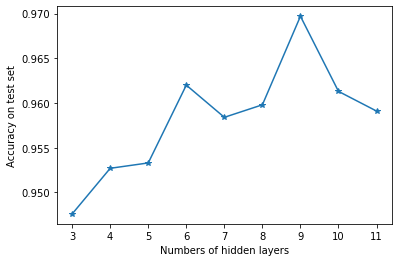
\includegraphics[width=0.7\textwidth,height=0.5\textwidth]{1.png}
	\caption{Accuracy varies with depth}
\end{figure}
\textbf{可以看出,在实验开始时,测试集上的精确率随着网络深度的增加而增大,并在网络深度达到$6$层时达到最大,这是因为随着深度的
增大,网络的参数量增加,网络的性能更好,对数据的拟合效果也会更好.但是随着深度的继续增加,网络的精确率出现先减小后增大最后又减小
的情况,这里尝试给出解释:网络精确率的第一次下降可能是由于随机初始化的影响,因为此时精确率并没有下降太多且很快出现回升态势,而网络
精确率的上升是因为深度的进一步增加使得参数进一步增多,网络的性能进一步增强,并在层数达到$9$时达到最大;最后再层数超过$9$后,由于
参数量过多,网络开始出现过拟合的现象,从而在测试集上的精确率开始降低.从本次实验中可以得到这样一个启示,即不可过分追求网络深度,要结合
数据集的特点,选择合适深度的网络,或者进行过合理的网络架构搜索,以选取最优的网络架构.}
\section{Ex2}
\par 对于第二问,这里对三种不同的网络架构,研究宽度对其分别的影响,为保证实验结果不受深度影响,这里分别固定其深度,每次改变全连接层
的宽度,以探究不同参数量下的网络精确率的变化,并可以得到分类准确率如下图(具体代码见fcn\_and\_cnn.py):
\begin{figure}[H]
	\centering
	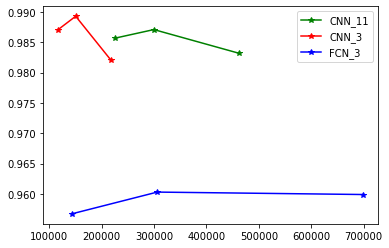
\includegraphics[width=0.7\textwidth,height=0.5\textwidth]{2.png}
	\caption{Accuracy varies with width}
\end{figure}
\textbf{可以看出,对于三种网络,均呈现出随着参数量增加,网络在测试集上的精确率先增后降的态势,这与Ex1中的分析类似,是因为网络随着参数量
的增加性能先是增强,而后出现过拟合导致的.再比较三种网络之间的差异,可以看出CNN的表现明显由于FCN,这是因为CNN的卷积操作,保留了图像的局部
结构信息,更适合处理图像信息,而FCN直接对图像的矩阵进行向量化操作(即"拉平"),会导致图像局部信息的丢失.而同样是CNN,$3$层卷积网络的性能
甚至要优于$11$层网络,这一点较为反常,这里尝试给出解释:因为MNIST数据集中的图片像素为$28\times 28$,尽管在程序中采取了类似LeNET中的
Resize操作将其重塑为$32\times 32$的图像,但是其尺寸仍旧较小,随着卷积操作和池化操作的不断进行,图像的尺寸不断缩小,进而图像的特征不
断缩小,最终导致网络抽取捕捉的特征相对较少,也就导致了网络的性能较$3$层卷积网络稍差.但是尽管如此,可以看出$11$层卷积网络的对于参数量或者
说宽度的鲁棒性较$3$层卷积网络更好,这是因为网络的深度更大,从而对于宽度的改变相对没有那么敏感,或者说更深的网络对于参数改变的影响更"光滑".}

\newpage
\begin{thebibliography}{3}  
	\bibitem{ref1} 李航. 统计学习方法[M]. 清华大学出版社, 2012.
	%\bibitem{ref2} Kingma D , Ba J . Adam: A Method for Stochastic Optimization[J]. Computer Science, %2014.
	\bibitem{ref2} Goodfellow, Ian, et al. Deep Learning[M]. MIT Press, 2016. 	
	\bibitem{ref3} Peter Harrington, 李锐 … [等. 机器学习实战[M]. 人民邮电出版社, 2013.
\end{thebibliography}
\end{document}
